\documentclass{beamer}
\usetheme{Boadilla}

%\usecolortheme{crane}
\usecolortheme{default}

\usepackage[english]{babel}
\usepackage[utf8x]{inputenc}
\usepackage{pifont}
\usepackage{pdfpages}
\usepackage{amsfonts}
\usepackage{dsfont}
\usepackage{amsmath}
\usepackage{amssymb}
%\usepackage{amsthm}
%\usepackage{natbib}
%\usepackage{hyperref}
\usepackage{bm}
\usepackage{xcolor}
\usepackage{caption}
%\usepackage{enumitem}
\usepackage{algorithm2e}
\usepackage[all]{xy} 
%\captionsetup[figure]{labelformat=empty}% redefines the caption setup of the figures environment in the beamer class.
\usepackage[absolute,showboxes,overlay]{textpos} % For textblocks
\TPshowboxesfalse %
\usepackage{array}



\newcommand*{\TakeFourierOrnament}[1]{{%
\fontencoding{U}\fontfamily{futs}\selectfont\char#1}}
\newcommand*{\danger}{\TakeFourierOrnament{66}}
\usepackage{caption}
\captionsetup[figure]{labelformat=empty}% redefines the caption setup of the figures environment in the beamer class so that "figure" does not display.

%
% %%%%% Etat des objets caches
% \setbeamercovered{transparent=02}
\setbeamercovered{transparent}

%\setbeamercolor{math text}{fg=blue}
% \useinnertheme{rectanglOes}

%%%%% Selection des symboles de navigation
%\setbeamertemplate{navigation symbols}{\insertframenavigationsymbol,
                                      % \insertbackfindforwardnavigationsymbol}
\setbeamertemplate{navigation symbols}{\insertframenavigationsymbol}


\titlegraphic{
\footnotesize
  %vincent.leclere@enpc.fr

  % EasyChair Preprint no. 4113, 2020.
  % \url{https://easychair.org/publications/preprint/pFGX}.

% \vspace{-1.5cm}

\includegraphics[width=6cm]{images/logo_UFR_Nantes_U.png}

}



%\newcommand{\mf}[1]{ }
%\newcommand{\mf}[1]{\begin{color}{blue}\tiny{mf: #1}\end{color}}


%\renewcommand{\va}[1]{\mathbf{#1}}


\newcommand{\red}[1]{\begin{color}{red}#1\end{color}}

\newcommand{\green}[1]{\begin{color}{green!70!black}#1\end{color}}
\newcommand{\orange}[1]{\begin{color}{orange!70!black}#1\end{color}}
\newcommand{\blue}[1]{\begin{color}{blue}#1\end{color}}
\newcommand{\magenta}[1]{\begin{color}{magenta}#1\end{color}}
\newcommand{\violet}[1]{\begin{color}{violet}#1\end{color}}
\newcommand{\brown}[1]{\begin{color}{brown}#1\end{color}}
\newcommand{\white}[1]{\begin{color}{white}#1\end{color}}
\newcommand{\yellow}[1]{\begin{color}{yellow!80!black}#1\end{color}}
\newcommand{\black}[1]{\begin{color}{black}#1\end{color}}

\newcommand{\imp}[1]{\blue{#1}}

\newcommand{\boldcheckmark}{\green{\ding{52}}}
\newcommand{\crossmark}{\red{\ding{54}}}

\newcommand\blfootnote[1]{%
  \begingroup
  \renewcommand\thefootnote{}\footnote{#1}%
  \addtocounter{footnote}{-1}%
  \endgroup
}

%%%%%%%%%%%%%%%%%%%%%%%%%%%%%%%%%%%%%%%%%%%%%%%%%%%%%%%%%%%%%%%%%%%%
%%%%%                                                          %%%%%
%%%%% Table des matières en début de section                   %%%%%
%%%%%                                                          %%%%%
%%%%%%%%%%%%%%%%%%%%%%%%%%%%%%%%%%%%%%%%%%%%%%%%%%%%%%%%%%%%%%%%%%%%

\AtBeginSubsection[]
{
  \begin{frame}<beamer>
    \frametitle{Sommaire}
    \addtocounter{framenumber}{-1}
    \tableofcontents[currentsection,currentsubsection]
  \end{frame}
}

\AtBeginSection[]
{
  \begin{frame}<beamer>
    \frametitle{Sommaire}
    \addtocounter{framenumber}{-1}
    \tableofcontents[currentsection]
  \end{frame}
}



\usepackage{xcolor}
\usepackage{tikz}
\usetikzlibrary{calc}
\usetikzlibrary{intersections}
\tikzset{offset/.style={to path={%
    -- ($(\tikztostart)!#1cm!(\tikztotarget)$)}},
         offset/.default=1}
\tikzset{>=latex}
\usepackage{tikz-3dplot}
\usepackage{pgfplots}
\usepackage{adjustbox}

\def\colorpoly{red!80!white}
\def\colorfiber{red!80!white}
\def\colorchcmplx{orange!90!black}
\def\legendabscisse{y_1}
\def\legendordonnee{y_2}
\def\costoriginx{0.7}
\def\costoriginy{0.7}
\def\costxlegend{-c_1}
\def\costylegend{-c_2}
\def\colorchamber{orange}
\def\colorFprime{violet}
\def\xminus{x}
\def\xplus{y}



\usepackage{appendixnumberbeamer}

\begin{document}





\title{Maths, Economie et Transition écologique}
\author[Maël Forcier]{Maël Forcier}
\date[28/11/2024]{
\small{
28 Novembre 2024} }

\maketitle


\newtheorem{prop}{Proposition}
\newtheorem{hypo}{Hypothesis}
\newtheorem{defi}{Definition}
\newtheorem{nota}{Notation}
\newtheorem{genform}{General Form}


\section{Rappels sur le réchauffement climatique et le GIEC}

  

\begin{frame}{Changement climatique selon le réchauffement moyen}
\centering
\includegraphics[scale=0.34]{images/Temperature.png}
\\
\tiny{Source : Figure RID.5(b), Résumé à l'intention des décideurs,
 6ème rapport du GIEC, Groupe de travail I}
\end{frame}

\begin{frame}{Plusieurs scénarios possibles}
\centering
\includegraphics[scale=0.41]{images/IPCC_scenarios.png}
\\
\tiny{Source : Figure RID.8(b), Résumé à l'intention des décideurs,
 6ème rapport du GIEC, Groupe de travail I}
\end{frame}


\begin{frame}{Lien entre GES et température}
\centering
\includegraphics[scale=0.3]{images/Lien_GES_Temperature.png}
\\
\tiny{Source : Figure RID.10, Résumé à l'intention des décideurs,
 6ème rapport du GIEC, Groupe de travail I}
\end{frame}


\begin{frame}
\frametitle{Les 3 groupes de travail du GIEC}

\begin{columns}
  \begin{column}{0.2\textwidth}
Groupe de travail I : 
\end{column}
\begin{column}{0.55\textwidth}
Les bases scientifiques physiques
\end{column}
\begin{column}{0.2\textwidth}
  \includegraphics[scale=0.07]{images/IPCC_AR6_WGI.jpg}
\end{column}
\end{columns}
\vspace{0.3cm}
\begin{columns}
  \begin{column}{0.2\textwidth}
Groupe de travail II : 
\end{column}
\begin{column}{0.55\textwidth}
Impacts, adaptation et vulnérabilité
\end{column}
\begin{column}{0.2\textwidth}
  \includegraphics[scale=0.073]{images/IPCC_AR6_WGII.jpg}
\end{column}
\end{columns}
\vspace{0.3cm}
\begin{columns}
  \begin{column}{0.2\textwidth}
Groupe de travail III : 
\end{column}
\begin{column}{0.55\textwidth}
Atténuation du changement climatique
\end{column}
\begin{column}{0.2\textwidth}
  \includegraphics[scale=0.126]{images/IPCC_AR6_WGIII.png}
\end{column}
\end{columns}

\
\end{frame}


\begin{frame}{Groupe 2 : Impacts, adaptation et vulnérabilité}
\centering
\includegraphics[scale=0.24]{images/Health_adaptation.png}
\includegraphics[scale=0.24]{images/Legend_impact_adaptation.png}
\\
\tiny{Source : Figure SPM.3(e), 
 6ème rapport du GIEC, Groupe de travail II}
\end{frame}

\section{Comment compter les émissions de gaz à effet de serre aujourd'hui ?}

% \begin{frame}{Citepa l'Insee des polluants et des GES}\url{https://www.citepa.org/wp-content/uploads/publications/ominea/OMINEA_2024.pdf}
% \end{frame}

\begin{frame}{Potentiel de réchauffement global (PRG)}
\centering
\includegraphics[scale=0.35]{images/PRG.png}
\end{frame}

\begin{frame}{Energies fossiles}

\begin{columns}
  \begin{column}{0.15\textwidth}
Charbon
\end{column}
\begin{column}{0.3\textwidth}
0,35 $kgCO_2 eq/kWh$
\end{column}
\begin{column}{0.25\textwidth}
  \includegraphics[scale=0.37]{images/charbon.jpeg}
\end{column}
\begin{column}{0.15\textwidth}
Electricité
\end{column}
\end{columns}
\vspace{0.3cm}
\begin{columns}
  \begin{column}{0.15\textwidth}
Pétrole
\end{column}
\begin{column}{0.3\textwidth}
0,26 $kgCO_2 eq/kWh$
\end{column}
\begin{column}{0.25\textwidth}
  \includegraphics[scale=0.08]{images/petrole.jpg}
\end{column}
\begin{column}{0.15\textwidth}
Transport
\end{column}
\end{columns}
\vspace{0.3cm}
\begin{columns}
  \begin{column}{0.15\textwidth}
Gaz
\end{column}
\begin{column}{0.3\textwidth}
0,20 $kgCO_2 eq/kWh$
\end{column}
\begin{column}{0.25\textwidth}
  \includegraphics[scale=0.088]{images/gaz.jpeg}
\end{column}
\begin{column}{0.15\textwidth}
Electricité\\ Bâtiment
\end{column}
\end{columns}
\end{frame}

\begin{frame}{Production de l'électricité}
\begin{columns}
  \begin{column}{0.26\textwidth}
Centrale à charbon\\
820 $kgCO_2/MWh$
\end{column}
\begin{column}{0.2\textwidth}
  \includegraphics[scale=0.15]{images/centrale_charbon.png}
\end{column}
\begin{column}{0.25\textwidth}
Photovoltaïque\\
44 $kgCO_2/MWh$
\end{column}
\begin{column}{0.2\textwidth}
  \includegraphics[scale=0.1]{images/PV.jpeg}
\end{column}
\end{columns}
\vspace{0.2cm}
\begin{columns}
  \begin{column}{0.26\textwidth}
Centrale à gaz\\
490 $kgCO_2/MWh$
\end{column}
\begin{column}{0.2\textwidth}
\centering
  \includegraphics[scale=0.14]{images/centrale_gaz.png}
\end{column}
\begin{column}{0.25\textwidth}
Eolien\\
11 $kgCO_2/MWh$
\end{column}
\begin{column}{0.2\textwidth}
\centering
  \includegraphics[scale=0.12]{images/eolienne.jpg}
\end{column}
\end{columns}
\vspace{0.3cm}
\begin{columns}
  \begin{column}{0.26\textwidth}
Centrale nucléaire\\
12 $kgCO_2/MWh$
\end{column}
\begin{column}{0.2\textwidth}
  \includegraphics[scale=0.04]{images/centrale_nucleaire.jpg}
\end{column}
\begin{column}{0.25\textwidth}
Hydroélectricité\\
24 $kgCO_2/MWh$
\end{column}
\begin{column}{0.2\textwidth}
  \includegraphics[scale=0.1]{images/3_gorges.jpg}
\end{column}
\end{columns}
\end{frame}

\begin{frame}{Electricité selon différents pays}
\begin{tabular}{c|c|c|c|c|c}
 & France & Brésil & Chine & Chine &Facteurs\\
 &2022 & 2021 & 1990 & 2022 &  d'émissions \\
 & & & & & ($kgCO_2/MWh)$\\ \hline
Charbon &1,2 \% & 3,7 \% & 72,2 \% & 61,7 \% & 820 \\ 
Pétrole &1,4 \% & 3,1 \% & 7,8 \% & 0,1 \% & 650 \\
Gaz &9,5 \% & 13,3 \% & 0,4 \% & 3,0 \% & 490 \\
Nucléaire & 62,0 \% & 2,2 \% & 0 \% & 4,7 \% & 12 \\
Hydroélectricité & 10,7 \% & 55,3 \% & 19,5 \% & 15,1 \% & 24\\
 Eolien &8,0 \% & 11,0 \% & 0 \% & 8,5 \% & 11\\
  PV &4,3 \% &2,6 \% & 0 \% & 4,8 \% & 44\\
  Biomasse & 1,7 \% &8,5 \% & 2,4 \% & 2,0 \% & 0 \\ 
  Autres & 1,2 \% & 0,30 \% & 0,1 \% & 0,1 \% \\\hline
  Facteur & & & & \\
  d'émissions & 79 & 132 & 650 & 529 \\
  ($kgCO_2/MWh$) & & & &
\end{tabular}

\end{frame}

\begin{frame}{Différentes comptabilités énergétiques}
\centering
\includegraphics[scale=0.18]{images/energies_reveilleur.png}
\footnotesize{Source : Le Réveilleur, Taux de retour énergétique : J.M. Jancovici dans l'erreur ?}
\end{frame}



\section{Modèles d'évalutions intégrés}

\begin{frame}{Différents type de modèle}
\begin{itemize}
 \item Modèles Top-down vs Bottom-Up
 \item Modèles statiques vs dynamiques
 \item Modèles d'optimisation
 \item Modèles déterministes vs stochastiques
 \item Variables : exogènes, endogène, contrôlées, stochastiques
\end{itemize}
\end{frame}



\begin{frame}
\frametitle{Equation de Kaya}
\begin{equation*}
GES=POP \times \frac{PIB}{POP} \times \frac{Energie}{PIB}\times \frac{GES}{Energie}
\end{equation*}
\pause
Modèle Top-Down très simplifié
\end{frame}

\begin{frame}
\frametitle{Modèle Bottom-Up : exemple du parc de logement}
\center{38 millions de logements \\
82 \% de résidences principales\\ 10 \% de résidences secondaires, 8 \% de logements vacants}
\vspace{0,2cm}
\begin{columns}
  \begin{column}{0.6\textwidth}
Maisons individuelles 54,8 \%

  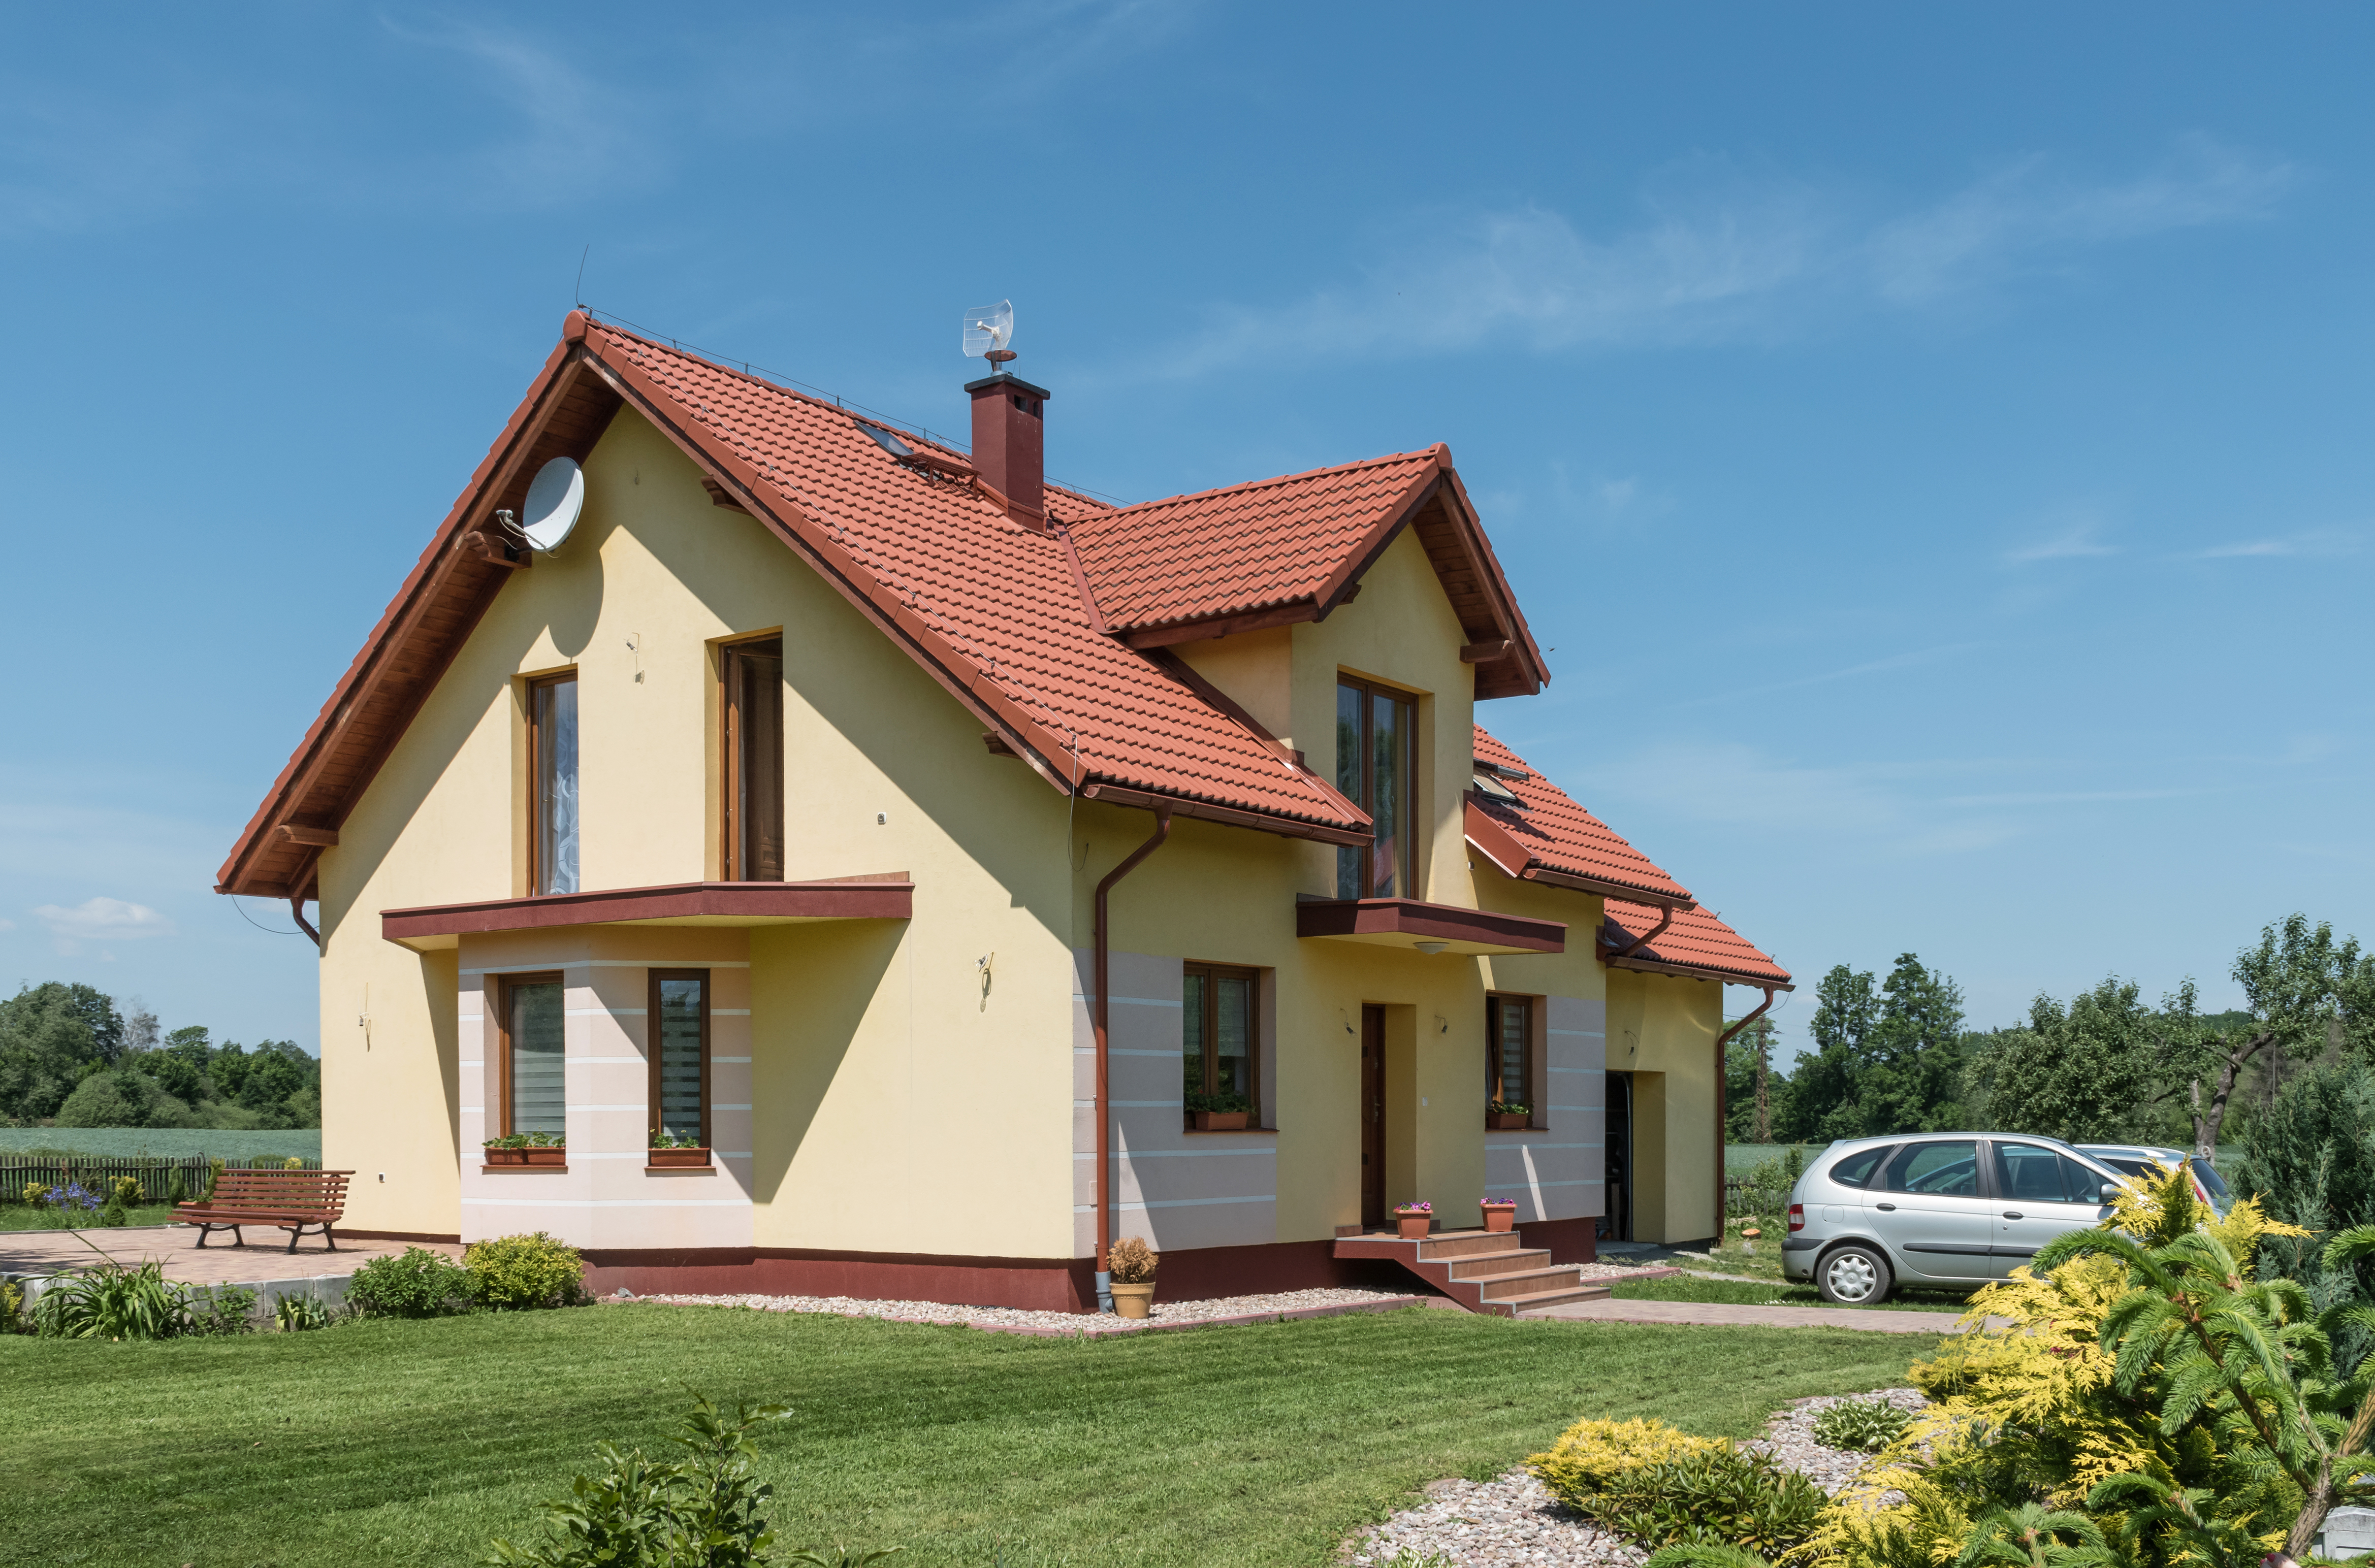
\includegraphics[scale=0.11]{images/maison_individuelle.jpg}
\end{column}
\begin{column}{0.4\textwidth}
Logements collectifs 45,2 \%

  \includegraphics[scale=0.12]{images/batiment_collectif.jpg}
\end{column}
\end{columns}
\vspace{0.5cm}
Résidences principales par énergie de chauffage
\vspace{0.3cm}
\small{
\begin{tabular}{c|c|c|c|c}
& Electricité & Gaz & Fioul & Bois et \\
& dont PAC & & et autres &réseau de chaleur \\ \hline 
Millions de logements & 11,47 & 10,84 & 3,08 & 4,83\\
Pourcentage & 38,0 \% & 35,9 \% & 10,2 \% & 16,0 \%
\end{tabular}
}
\end{frame}


 \begin{frame}
\frametitle{Modèle Bottom-Up : exemple du parc de véhicules}
\center{46 millions de véhicules}
\vspace{0,5cm}
\begin{columns}
  \begin{column}{0.5\textwidth}
  Voiture thermique
  \includegraphics[scale=0.43]{images/essence.jpg}
\end{column}
\begin{column}{0.5\textwidth}
Voiture électrique
\includegraphics[scale=0.037]{images/voiture_electrique.JPG}
\end{column}
\end{columns}


\end{frame}


\begin{frame}{World 3 (1972)}

\begin{columns}
  \begin{column}{0.5\textwidth}

  \center{ 
  \includegraphics[scale=0.1]{images/limits_to_growth.png}\\\small{Les limites à la croissance, premier rapport du Club de Rome}
  \vspace{0,5cm}
   
\includegraphics[scale=0.6]{images/equipe_meadows.jpg}
\\
\small{Jorgen Randers, Jay Forrester, Donella et Dennis Meadows, William W. Behrens}.
}
  
\end{column}

\begin{column}{0.5\textwidth}  
\includegraphics[scale=0.2]{images/limits-to-growth-figure.png}
\end{column}
\end{columns}
\end{frame}



\begin{frame}{DICE, Dynamic Integrated Climate Economy (1992)}
\begin{columns}
  \begin{column}{0.7\textwidth}
  
  2018 : Prix de la Banque de Suède en sciences économiques en mémoire d'Alfred Nobel \\
  \vspace{0,5cm}
  ``Pour avoir intégré le changement climatique dans l'analyse macroéconomique de long terme.''
\end{column}

\begin{column}{0.3\textwidth}

\center{
\includegraphics[scale=0.15]{images/Nordhaus.jpg}
\\
William D. Nordhaus}
\end{column}
\end{columns}
\center{
\includegraphics[scale=0.23]{images/DICE_Fig3_Legend.png}}

\end{frame}



\end{document}